\documentclass{beamer}
\beamertemplatenavigationsymbolsempty
\usecolortheme{beaver}
\setbeamertemplate{blocks}[rounded=true, shadow=true]
\setbeamertemplate{footline}[page number]
%
\usepackage[utf8]{inputenc}
\usepackage[english]{babel}
\usepackage{amssymb,amsfonts,amsmath,mathtext}
\usepackage{subfig}
\usepackage[all]{xy} % xy package for diagrams
\usepackage{array}
\usepackage{multicol}% many columns in slide
\usepackage{hyperref}% urls
\usepackage{hhline}%tables
% Your figures are here:
\graphicspath{ {fig/} {../fig/} }

%--------------------------------------------------------------------------------------------------

\title[\hbox to 56mm{Detecting Alterations}]{Detecting Manual Alterations in Biological Image Data Using Contrastive Learning and Pairwise Image Comparison}
\author[G.\,S.~Nekhoroshkov]{Georgii Nekhoroshkov}
\institute{Moscow Institute of Physics and Technology}
\date{\footnotesize
\par\smallskip\emph{Course:} My first scientific paper\par (Strijov's practice)
\par\smallskip\emph{Expert:} A.\,V.~Grabovoy
\par\smallskip\emph{Consultant:} D.\,D.~Dorin
\par\bigskip\small 2025}

%--------------------------------------------------------------------------------------------------

\begin{document}

%--------------------------------------------------------------------------------------------------

\begin{frame}
\thispagestyle{empty}
\maketitle
\end{frame}

%--------------------------------------------------------------------------------------------------

\begin{frame}{Goal of research}
\begin{block}{Ensure biological image integrity}
Develop a contrastive learning model for pairwise image comparison to:
\begin{itemize}
    \item Detect alterations (color jittering, crop, rotation, noise) 
    \item Select pairs of images with the same content
    \item Outperform existing state-of-the-art  models (Barlow Twins\footnote{{\tiny \textit{J. Zbontar et al.} Barlow Twins: Self-Supervised Learning via Redundancy Reduction // ICML, 2021.}}, SimCLR\footnote{{\tiny \textit{T. Chen et al.} A Simple Framework for Contrastive Learning of Visual Representations // ICML, 2021.}}) on cell datasets
\end{itemize}
\end{block}
\begin{center}
    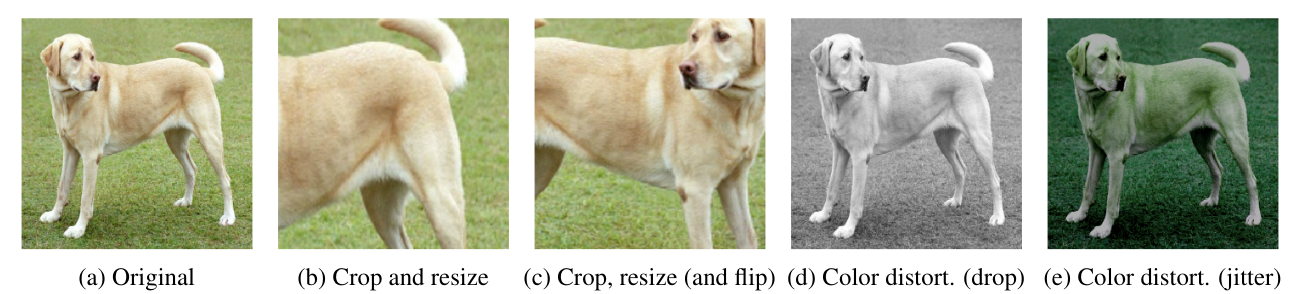
\includegraphics[width=1\textwidth]{fig/alterations.png}
\end{center}
\end{frame}

%--------------------------------------------------------------------------------------------------

\begin{frame}{One-slide talk}
\begin{block}{The problem}
Detection of similar images despite modifications.
\end{block}

\medskip

\begin{columns}
    \begin{column}{0.42\textwidth}
        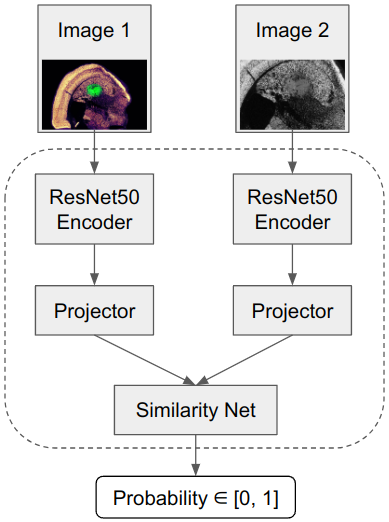
\includegraphics[width=0.86\textwidth]{fig/model.png}
    \end{column}
    \begin{column}{0.58\textwidth}
        The model should process two images and output a value from [0, 1] --
        the likelihood that they are identical, up to modifications.
        
        \bigskip
        The method must leverage a self-supervised learning approach.
    \end{column}
\end{columns}
\end{frame}

%--------------------------------------------------------------------------------------------------

\begin{frame}{Literature}
\begin{block}{Key Articles}
    \begin{itemize}
        \item \textbf{SimCLR}: Chen T. et al. "A Simple Framework for Contrastive Learning of Visual Representations", ICML 2020
        \item \textbf{Barlow Twins}: Zbontar J. et al. "Barlow Twins: Self-Supervised Learning via Redundancy Reduction", ICML 2021  
        \item \textbf{CLIP}: Radford A. et al. "Learning Transferable Visual Models From Natural Language Supervision", ICML 2021
        \item \textbf{Siamese Networks}: Melekhov I. et al. "Siamese Network Features for Image Matching", ICPR 2016
    \end{itemize}
\end{block}
\end{frame}

%--------------------------------------------------------------------------------------------------

\begin{frame}{Problem statement}
\begin{block}{Given biological image dataset}
    \begin{equation*}
        \mathcal{D} = \{d_i \in \mathcal{S},\ i \in [0, N)\},\quad 
        \mathcal{S} \subseteq \mathbb{R}^{H \times W \times C}
    \end{equation*}
\end{block}

\begin{block}{Pairwise similarity classification}
    For any $(x, y) \in \mathcal{S} \times \mathcal{S}$, learn mapping:
    \begin{equation*}
        \mathcal{M}: (x, y) \mapsto s \in [0, 1]
    \end{equation*}
    where:
    \begin{itemize}
        \item $s=1$: \textit{similar} pair (same content pre-alteration)
        \item $s=0$: \textit{dissimilar} pair (different content)
    \end{itemize}
\end{block}
\end{frame}

%----------------------------------------------------------------------------------------------------

\begin{frame}{Problem statement}
\begin{block}{Model decomposition}
    $$ \mathcal{M}(x, y) = h(f(x), f(y)) $$
    where:
    $$ f : \mathcal{S} \rightarrow \mathbb{R}^d \, \text{(encoder)} $$
    $$ h : \mathbb{R}^d \times \mathbb{R}^d \rightarrow [0, 1] \, \text{(classifier)} $$
\end{block}

\begin{block}{Success criterion}
    Maximize accuracy over pairwise comparisons:
    \begin{equation*}
    \text{Acc} = \frac{1}{|\mathcal{P}|} \sum_{(x,y) \in \mathcal{P}} \mathbb{I}\big(\mathcal{M}(x,y) = I(x,y)\big)
    \end{equation*}
    where $\mathcal{P}$ is test pairs, $I(x,y)$ ground truth similarity.
\end{block}
\end{frame}

%-----------------------------------------------------------------------------------------------------

\begin{frame}{Solution}
\begin{columns}
    \column{0.53\textwidth}
    \begin{block}{Barlow Twins Adaptation}
        \vspace{3mm}
        Architecture:
        \begin{itemize}
            \item ResNet-50 backbone
            \item Projector
            \item Similarity head
        \end{itemize}
        Training specific:
        \begin{itemize}
            \item Parallel image augmentation
            \item AdamW optimizer with decreasing learning rate
            \item Performed on a specially selected dataset
        \end{itemize}
        
        \vspace{2mm}
        \textbf{Key Innovation:} \\
        Custom model's head and dataset \\
    \end{block}
    
    \column{0.52\textwidth}
    \begin{center}
        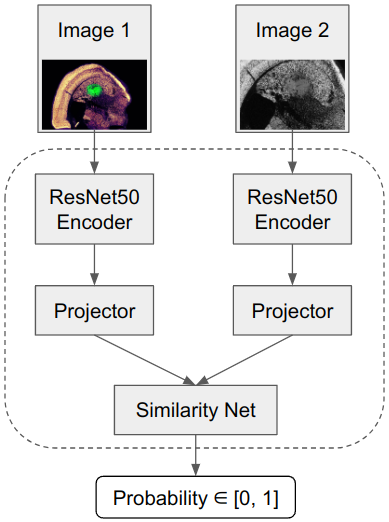
\includegraphics[width=1\textwidth]{fig/model.png}
    \end{center}
\end{columns}
\end{frame}

%--------------------------------------------------------------------------------------------------

\begin{frame}{Computational experiment}
\begin{block}{Experimental Setup}
\begin{itemize}
    \item \textbf{Dataset}: 630 biological scans (animal and plant cells)
    \item \textbf{Train/Test Split}: 80\%/20\%
    \item \textbf{Training}: 100 epochs, AdamW optimizer ($\gamma_{start}=3\cdot10^{-3}, \gamma_{end}=5\cdot10^{-4}$)
\end{itemize}
\end{block}

\begin{block}{Evaluation Protocol}
\begin{itemize}
    \item Compare with Barlow Twins baseline
    \item Metrics:
    \begin{itemize}
        \item Accuracy 
        \item F1-Score, Precision, Recall
        \item AUC-ROC
    \end{itemize}
\end{itemize}
\end{block}
\end{frame}

%--------------------------------------------------------------------------------------------------

\begin{frame}{Computational Experiment}
\begin{columns}[T]
    \column{0.50\textwidth}
    \vspace{-4mm}
    \begin{block}{ROC-AUC Comparison}
        \centering
        \vspace{-2mm}
        {\tiny Model} \\
        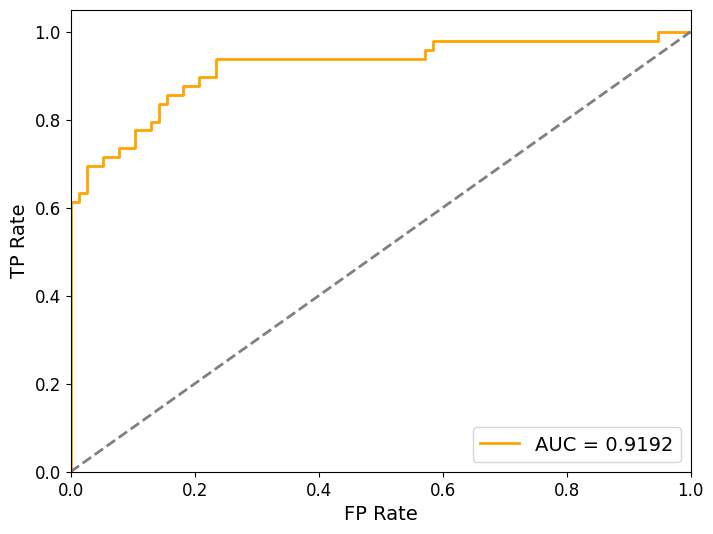
\includegraphics[width=0.9\textwidth]{fig/roc-curve-model.png} \\
        \vspace{-2mm}
        {\tiny Barlow Twins} \\
        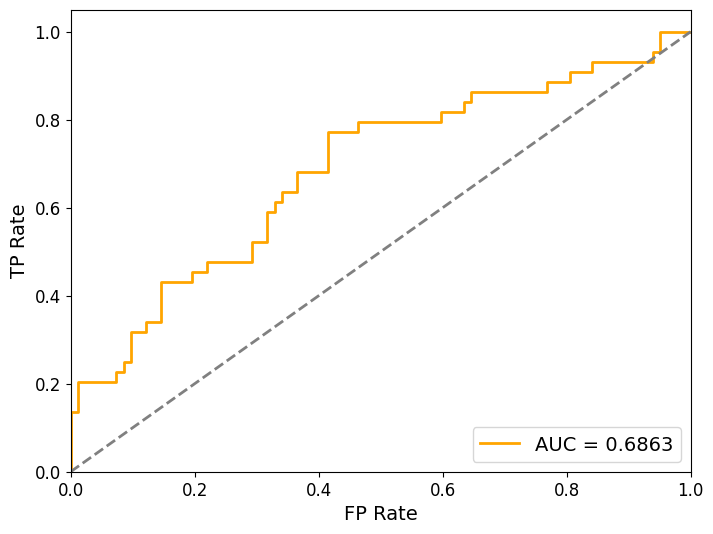
\includegraphics[width=0.9\textwidth]{fig/roc-curve-BT.png}
    \end{block}

    \column{0.50\textwidth}
    \vspace{-4mm}
    \begin{block}{Performance Metrics}
        \vspace{3mm}
        \centering
        \begin{tabular}{lcc}
        \hline
        Metric & Model & Barlow Twins \\ \hline
        Accuracy & \color{red}0.85 & 0.68 \\
        F1-Score & \color{red}0.80 & 0.48 \\
        Precision & \color{red}0.82 & 0.54 \\
        Recall & \color{red}0.78 & 0.43 \\ 
        AUC & \color{red}0.92 & 0.69 \\ \hline
        \end{tabular}
    \end{block}
    
    \begin{itemize}
        \footnotesize
        \item All metrics computed on test set (20\% data)
        \item Threshold = 0.5 for binary classification
    \end{itemize}
\end{columns}
\end{frame}

%--------------------------------------------------------------------------------------------------

\begin{frame}{Conclusion}
\begin{block}{Key achievements}
    \begin{itemize}
        \item Significant accuracy metrics improvement over state-of-the-art model
        \item Robust to 4 types of manual alterations
        \item First biological-SSL solution for:
        \begin{itemize}
            \item Automated fraud detection
            \item Image provenance verification
        \end{itemize}
    \end{itemize}
\end{block}
\end{frame}

\end{document}
